\section{Kriteriji za klasifikacijo spletnih portalov}
\label{sec:kriteriji_za_klasifikacijo_spletnih_portalov}

Spletni portali imajo različne značilnosti in zmožnost. V poglavju
bomo razdelali posamezne kriterije s katerimi bomo klasificirali in
ovrednotili posamezne spletne portale.

\subsection{Vrsta vsebine}
\label{sec:Razvrstitev_spletnih_portalov}

Po hitrem pregledu in iskanju spletnih portalov lahko ugotovimo, da
spletni portalu za učenje programiranja ponujajo najrazličnejše vrste
vsebin in njihove kombinacije kot je na primer, \textbf{tekstovni
  vodič in spletno aplikacija za programiranje}. V posebno kategorijo
bomo uvrstili tudi spletne portale, ki ponujajo \textbf{spletne igre},
ki učijo programiranje. Različne vrste spletnih portalov, ki jih lahko
obravnavamo so naslednje:

\begin{itemize}
\tightlist
\item \textbf{tekstovni vodič}i,
\item \textbf{video vodič},

\item \textbf{spletna aplikacija za programiranje}, kot smo jo
  definirali v poglavju \ref{sec:značilnosti_spup},
\item \textbf{spletne igre},
\item \textbf{kombinacija} vrst vsebin, ki jih lahko še razdelimo na:
  \begin{itemize}
    \tightlist
  \item \textbf{najosnovnejša kombinacija} (\emph{tekstovni vodič + preizkus kode});
  \item \textbf{napredna kombinacija} (\emph{različne vrste vodičev +
      spletna aplikacija za programiranje}).
  \end{itemize}
\end{itemize}

V tej diplomi se ne bomo specifično ukvarjali s tem katera izmed vrst
vsebin predstavlja boljše zmožnosti za prenos znanja. Vsaka ima svoje
prednosti in slabosti, zato bomo za vsako izpostavili njene pozitivne
značilnosti tudi slabosti. Zanimale nas bodo predvsem tise
\textbf{kombinirane} vrste vsebin, ki bodo predstavljale čim bolj
celovit spletni portal za učenje programiranja, kot smo ga definirali
v poglavju \ref{sec:značilnosti_spup}.

%Kje naredim razdelek med spletnim portalom z vsebino in tistim, ki
%ponuja razvojno okolje in služi le kot orodje za preizkus programske
%kode in potrebuje da učitelj sam doda vsebino.

\subsubsection{Tekstovni vodiči}

Spletni vodiči so najstarejša metoda podajanja znanja. Spletni vodiči
imajo značilnost, da uporabnika vodijo \textbf{po koraki}h do nekega
določenega cilja. Besedilo, ki podaja znanje je opremljeno z
\textbf{primeri}. \cite{wiki:tutorials}

Značilni predstavniki takih vodičev je spletna stran
\url{https://docs.python.org} na kateri najdemo vso dokumentacijo
programskega jezika \textbf{Python}. Na strani najdemo tudi vodiča z
naslovom \emph{\href{https://docs.python.org/3/tutorial/index.html}{The
  Python Tutorial}} \cite{web:TPythonTut The}.

\begin{figure}[h!]
    \includegraphics [width=1\linewidth, keepaspectratio =
    1] {./images/sc_web/tPyTut_01.png}
    \caption{Zaslonski posnetke poglavja z vodiča
      \emph{\href{https://docs.python.org/3/tutorial/index.html}{The
          Python Tutorial}} s primerom \cite{web:TPythonTut}.}
    \label{fig:scr:web:tPyTut}
\end{figure}

Spletne vodiče pri pouku uporabljamo na podoben način kot pri
\textbf{metodo dela s tekstom}. Sicer je pomembno da učenci usvojijo
uporabo spletnih vodičev, vendar so spletni vodiči marsikdaj
prezahtevni za uporabo sploh na osnovno šolskem nivoju. Negativna
stran spletnih vodičev je še ta, da direktno s spletne strani ne
moramo preizkušati primerov programske kode, kar je slabo tudi Z
motivacijskega vidika.

\subsubsection{Video vodiči}
\label{sec:video_vodici}

Z razmakom video vsebin na spletu, so marsikateri spletni vodič
dopolnili oz. zamenjali video vodiči. Popularno je postalo zajemanje
oz. \textbf{snemanje lastnega namizja}. Vido vodiče najdemo za
številna področja, od uporabe določene programske opreme in vse do
programiranja. Ena izmed prednosti video vodičev naprem tekstovnim je
ta, da ti omogočajo nazornejši prikaz nekega postopka. Preden sami
posnamemo nek postopek, lahko v video posnetku opazujemo vsak korak,
potek miške in poleg teka poslušamo razlago, če je ta vključena.
Številne študije kažejo da je učenje s multimedijo, torej kombinacijo
zvoka in slike dosti bolj učinkovito, samo poslušanje ali branje
teksta \cite{web:multimediaL}. V razredu je uporaba video vodičev
lahko koristna pri samostojnem delu in domačem delu. Uporaba video
vodičev ima tudi slabe strani, v njih lahko predstavimo dosti manj
vsebine in iskanje vsebine ni preprosto, kot je to pri tekstu.

Eden izmed spletnih portalov, ki je specializiran za podajanje znanja
s video vodiči je \emph{\href{https://www.udemy.com}{Udemy}}
\cite{web:udemy}. Na njem vsak kdo lahko postane učitelj in pripravi
učne ure z različnih področij, ne samo z računalniške
znanosti. Nekateri sklopi učnih ur so v celoti brezplačni, večin je
plačljivih.

\begin{figure}[h!]
    \includegraphics [width=1\linewidth, keepaspectratio =
    1] {./images/sc_web/udemy_01.png}
    \caption{Zaslonska slika spletne strani
      \emph{\href{https://www.udemy.com}{Udemy}}
      \cite{web:udemy}. Na prosto dostopnem sklopu učne ure v
      pythonu.}
    \label{fig:scr:web:udemy}
\end{figure}

\subsubsection{Spletna aplikacija za programiranje.}
\label{sec:spletna_app_programiranje}

Nekatere spletne strani ponujajo le spletno aplikacijo za
programiranje, kot smo jo povzeli v poglavju
\ref{sec:značilnosti_spup}. Taki spletni portali ne ponujajo vsebine,
ponujajo le \textbf{orodje}. Ali pa ponujajo le toliko vsebine, kot je
potrebno, da se uporabnik nauči uporabljati spletno aplikacijo. Kljub
temu, da nas zanimajo celoviti spletni portali, ki ponujajo tudi
vsebino, nas bodo podrobneje zanimala tudi orodja. Prednost uporabe
spletne aplikacij ali orodja je ta, da ima mentor (\emph{učitelj})
svobodno izbiro, katero vsebino bo podajal. Priprava vsebine sicer
terja več truda in časa mentorja, vendar lahko vsebino prilagaja in jo
prireja po potrebi.

Predstavnik takega orodja je
\emph{\href{http://pythonfiddle.com/}{Python Fiddle}}
\cite{web:pythonfiddle}. Omogoča osnovni urejevalnik besedila (slika), z
barvanjem programske kode, s predlogami za samo dokončevanja izpisa
vgrajenih funkcij. Uvozimo lahko datoteke in jih delimo. Zaganjamo
napisane programe, izhodni podatki se izpišejo v konzoli.

\begin{figure}[h!]
    \includegraphics [width=1\linewidth, keepaspectratio =
    1] {./images/sc_web/PythonFiddle_01.png}
    \caption{Zaslonska slika spletne applikacije za programiranje
      \emph{\href{http://pythonfiddle.com/}{Python Foddle}}
      \cite{web:pythonfiddle}.}
    \label{fig:scr:web:PyFiddle}
\end{figure}

Spletne tehnologije so danes zalo napredovale in že nekaj let se
aplikacije in podatki selijo v \textbf{oblak}. Te aplikacije in
podatki so dostopni od koder koli. V \textbf{oblaku} so razvijajo
številna profesionalna okolja \textbf{IDE}, ki omogočajo delo na
večjih projektih in ponujajo napredne funkcije IDE, ki smo jih drugače
lahko imeli le z namiznimi aplikacijami. Navedimo dva primera:
\emph{\href{https://codenvy.com/}{Codenvy}} \cite{web:codeenvy} in
\emph{\href{https://c9.io/}{Cloud9}}\cite{web:cloud9}. Oba ponujata
profesionalen IDE v oblaku. Za uporabo v šoli sta ti dve okolji preveč
zahtevni, in jih ni smiselno uporabljati pri poučevanju novincev. S
tem jim otežimo učenje programiranja, saj prej potrebujejo čas, da
spoznajo in se naučijo uporabljati IDE.

\subsubsection{Spletne igre}
\label{sec:spletne_igre}

Na spletu obstajajo številni spletni portali, ki učijo in spodbujajo k
učenju programiranja s igrami podobnimi vsebinami. Vsebina je
razdeljena na stopnje. Igralci na napreduje iz stopnje v stopnjo in
pri tem nabirajo izkušnje, nove veščine in dosežke. Za igranje igre ne
upravljamo z liki v igri z tipkovnico in miško temveč pišemo
programsko kodo, ki upravlja njihovo početje. Takšni spletni portali
dajejo zelo dobro motivacijsko osnovo, saj se novinci spoznajo na
osnovne principe igranja iger. Primer spletnega portala je
\emph{\href{http://fightcodegame.com/}{Fightcode}}
\cite{web:fightcode}. Igralci programirajo robota v programskem jeziku
JavaScript. Vsak izmed igralcev lahko izzove drugega igralca v boj med
roboti. Za vsako zmago se igralec pomika navzgor po lestvici
najboljših robotov.

\begin{figure}[h!]
    \includegraphics [width=1\linewidth, keepaspectratio =
    1] {./images/sc_web/fightRobot_01.png}
    \caption{Zaslonska slika spletne strani
      {\href{http://fightcodegame.com/}{Fightcode}}
      \cite{web:fightcode}.}
    \label{fig:scr:web:w3school}
\end{figure}

V podrobnem pregledu si bomo še podrobneje ogledali nekatere druge
spletne igre, ki učijo programirati.

\subsubsection{Kombinirane vrste vsebin}
\label{sec:kombinirane_vrste_vsebin}

V prejšnjih poglavjih smo opisali \textbf{osnove vrste} spletnih
portalov. Zanimale nas bodo predvsem \textbf{kombinirane vrste}, ki so
sestavljene iz osnovnih. Te bodo podale celovite portale. Na spletu
najdemo številne kombinacije spletnih portalov,\textbf{Osnovno
  kombinirano vsebino} predstavljajo spletni portali, kot je
\emph{\href{http://www.w3schools.com/}{w3School}}
\cite{web:w3school}. Sestavljeni so iz \textbf{tekstovnih vodičev} in
\textbf{najosnovnejšega preizkusa programske kode}. Vsak primer v
vodiču je opremljen s primerom, katerega lahko zaženemo in preizkusimo
kaj je rezultat primera. Za izvajanje primera pritisnemo na gumb
\textbf{Preizkusi!  (\emph{ang. Try it!})} Programsko kodo primera
lahko tudi spreminjamo in jo ponovno izvajamo.

\begin{figure}[h!]
    \includegraphics [width=1\linewidth, keepaspectratio =
    1] {./images/sc_web/w3school.png}
    \caption{Zaslonska slika spletne strani
      \emph{\href{http://www.w3schools.com/}{w3School}}
      \cite{web:w3school}.}
    \label{fig:scr:web:w3school}
\end{figure}

\textbf{Napredno kombinirano vsebino} predstavljajo spletni portali, ki so
sestavljeni \textbf{tekstovnega vodiča in/ali video vodičev ter
  spletne aplikacije za programiranje}. Omenimo naslednjega
predstavnika \emph{\href{https://www.codeschool.com/}{Codeschool}}
\cite{web:codeschool}.

\begin{figure}[h!]
    \includegraphics [width=1\linewidth, keepaspectratio =
    1] {./images/sc_web/codeschool_01.png}
    \caption{Zaslonska slika spletne strani
      \emph{\href{https://www.codeschool.com/}{Codeschool}}
      \cite{web:codeschool}.}
    \label{fig:scr:web:codeschool}
\end{figure}

Poleg različnih vrst vsebin imajo še druge zmožnosti, ki jih bomo
spoznali pri podrobnem pregledu.

\subsection{Jezik spletnega portala}
\label{sec:jezik_spletnega_portala}

Ugotovimo lahko, da večina spletnih portalov uporablja
\textbf{angleščino} kot primarni jezik. Nekateri ponujajo tudi druge
jezike, vendar je \textbf{slovenščina} zaradi majhnosti le malo krat
zajeta, razen v redkih primerih. Angleščina je glavni jezik spleta in
računalniške znanosti, zato je pomembno, da učenci oz. dijaki spoznajo
tudi angleške izraze in jih seveda povežejo s pravilnimi
slovenskimi. Kljub temu, da je učenje v slovenskem jeziku strogo
predpisano, lahko vsako učno uro s uporabo spletnih portalov za učenje
programiranja dobro povežemo med predmetno z angleščino.

%Kje je zapisano, načelo uporabe slovenščine. Kakšna je rešitev za
%uporabo spletne strani v tujem jeziku.

\subsection{Ponujena znanja}
\label{sec:vsebina_problemsk_pristop}

Spletne strani za učenje programiranje navadno ponujajo znanja oz
veščine programiranja z določenim programskim jezikom. Nekatera svojo
ponudbo širijo tako, da ponujajo številne druge projekte, ki
združujejo prej naučeno znanje. Na primer izdelava
\textbf{interaktiven spletne strani}. Za posamezen spletni portal nas
bo zanimalo ali ponuja samo:

\begin{itemize}
  \tightlist
\item \textbf{znanja/veščine programiranja} (programskega jezika) ali tudi,
\item \textbf{druga znanja/veščine} (npr. izdelava spletne strani).
\end{itemize}

% Zanimajo nas osnovna načela. -> Razdelaj na načela

\subsection{Programski jeziki}
\label{sec:_zanaja_programski_jeziki}

Zanimalo nas bo katere in koliko različnih programskih jezikov ponuja
nek spletni portal. Najbolj pogoste programske jezike smo opisali v
poglavju \ref{sec:programski_jeziki}, v prvi vrsti nas bodo zanimali
spletni portali, ki ponujajo te programske jezike. Prednost bodo imeli
tisti, ki ponujajo Python. Večina takšnih spletnih portalov ponuja več
programskih jezikov.

\subsection{Težavnostna stopnja}
\label{sec:težavnostna_stopnja}

Vsak spletni portal je namenjen svojemu občinstvu, zato se razlikujejo
se tudi po težavnostni stopnji, čeprav govorimo o novincih. Glavna
težavnostna razdelitev bo na \textbf{osnovo} in \textbf{srednjo
  šolo}. Po potrebi bomo podrobneje razdelili že osnovno šolo, ki je
razdeljena na triletja. Večina spletnih portalov izhaja iz Združenih
držav amerike, zato smo povzeli njihove stopnje šolanja
(\ref{tab:primerjava_šolski}), saj nekatere strani uporabljajo
\textbf{K-12} formulacijo za definicijo težavnosti oz. prilagoditev
učnemu načrtu. V podrobnem pregledu bomo ocenili, kateri težavnostni
stopnji ustreza spletni portal.

\begin{table}[!h]
\caption{Primerjava starosti in stopnje šolanja šolskega sistema v ZDA
  in Slovenskega \cite{wiki:k12}.}
\label{tab:primerjava_šolski}
\begin{tabular}{
  | p{0.33\linewidth-2\tabcolsep} |
  p{0.33\linewidth-2\tabcolsep} |
  p{0.33\linewidth-2\tabcolsep} |  }
\hline
  \rowcolor{sbase01!100}
  \textbf{Leta} & \textbf{Ang. K-12 naziv} & \textbf{SI Primerjava} \\
        \hline
      6 - 10    & \emph{Elementary school} & \textbf{1. in 2. triletje
                                             OŠ}\\
        \hline
      10 - 14    & \emph{Middle school} & \textbf{3. triletje OŠ} \\
        \hline
      10 - 14    & \emph{Highe school} & \textbf{Srednja šola} \\
  \hline
\end{tabular}
\end{table}

%Razdelaj načele problemski pristop. postopnosti in sistematičnosti.
\subsection{Upoštevanj načel}
\label{sec:upoštevanje_načel}

Za uspešno delo in uporabo SPUP v razredu je dobro, da vsebine, ki jih
najdemo na spletu sledijo \textbf{načelom}, ki jih upoštevamo tudi
drugače pri pouku.

\textbf{Problemski pristop}

Zanimalo nas bo ali spletni portal ponuja vsebine in ali so te
zasnovane problemsko. Glede vsebine se lahko sprašujemo naslednje.

\begin{itemize}
\tightlist
\item Ali spletni portali ponujajo vsebine računalniške znanosti?
\item Ali spletni portali ponujajo realne življenjske primere?
\item Ali so primeri problemsko zasnovani?
\item Ali je pomembno predvsem učenje programskega jezika?
\end{itemize}

\subsection{Uporaba ocenjevanja dosežkov značilnih za igre}
\label{sec:uporaba_dosežkov}

%ToDo: Slovenski izraz za Gamification.
V izobraževanju se uveljavlja trend ocenjevanja napredka in dosežkov,
ki je tipičen za video igre. To metodo ocenjevanje so poimenovali
\emph{ang. Gamification}. Vsako snov ali naloga, ki je v osnovi toga,
popestrimo z načinom ocenjevanja tako, da vsako nalogo predstavimo z
različnimi izzivi. Vsaki nalogi oz. izzivu sledijo različne nagrade,
ki jih učenci zbirajo in jim pravimo dosežki \cite{web:edublogger}.

Dosežki v video igrah so prisotni že vrsto let. Dosežki se razlikujejo
po kompleksnosti, vse od zmagoslavne glasbe ob končani stopnji ali
igri pa vse do kompleksnega sistema dosežkov, z zbiranjem
značk. Značko igralec dobi, ko na primer zbere dovolj predmetov ali
razišče določen procent ozemlja. Poznamo več načinov nagrajevanja
dosežkov. Kot smo že omenili lahko dosežke predstavimo kot
\textbf{značke} ali za posamezne izzive pripravimo sistem točkovanja,
ki se jih zbira. Z zbranih točk se lahko sestavijo \textbf{lestvice
  ali uvrstitev}. V razredu slednje morajo biti skrbno načrtovane, da
ne pride do prevelikih razlik med učenci in bi, kjer bi se eni lahko
počutili nadrejeni in drugi podrejene.

Zanimalo nas bo ali spletne portali, ki učijo programiranja
uporabljajo kakršen koli sistem ocenjevanja dosežkov, saj za tiste, ki
ga uporabljajo lahko rečemo, da imajo dodaten motivacijski faktor.

\subsection{Dodajanje lastnih vsebin}
\label{sec:dodajanje_vsebin}

Nekateri spletni portali omogočajo, da pripravimo lastne vsebine, ki
jih potem delimo. Navadno je \textbf{spletna aplikacija za
  programiranje} razširjena tako, da omogoča sestavljanje programskih
nalog. Večina teh je taka, da pripravimo \textbf{spremno besedilo,
  začetni program ali ogrodje programa, končno različico in pomoč ali
  namig}. Lahko so dodani tudi \textbf{testni vhodni in izhodni
  podatki}. Z podatki, ki smo jih vnesli imamo avtomatizirano nalogo,
ki jo lahko posredujemo oz. delimo z novincem. Zanimalo nas bo ali
kateri spletni portal omogoča to zmožnost.

\subsection{Upravljanje razreda}
\label{sec:upravljanje_razreda}

Zmožnost upravljanja razreda, je velika prednost in lajšanje dela pri
administraciji razreda za mentorja. Osnovni način delovanja je
naslednji. Mentor ustvari razred ali predmet, podobno kot je to možno
pri sistemih spletnih učilnic kot je
\emph{\href{https://moodle.org/}{moodle}} \cite{web:moodle_site}, v
učilnico povabimo učence in s tem na spletni portal. Učitelj s spletne
učilnice spremlja napredek in dosežke posameznega učenca. Spletni
portali spremljanje učencev navadno ponujajo kot plačljivo storitve za
šole, kar navadno ni najbolj poceni. Zanimalo nas bo ali spletni
portal ponuja \textbf{upravljanje razreda} in ali je ta storitev
\textbf{plačljiva ali brezplačna}.

\subsection{Dostop do gradiv}
\label{sec:dostop_do_gradiv}

Veliko vsebin na spletu je brezplačnih in jih v šolstvu lahko
uporabimo. Mnogo vsebin je tudi takšnih, ki jih je potrebno
plačati. Spletni portali, ki imajo plačljive vsebine uporabljajo
navadno model \textbf{plačevanja naročnine} za dostop do
vsebin. Uporabnik more na \textbf{letni ali mesečni} ravni odšteti
različne zneske. Nekateri izmed portalov, kot je \emph{Codeacademy}
imajo plačljive le nekatere zahtevnejše vsebine. Drugi portali imajo
vso vsebino ne dostopno. Obstaja tudi vrsta portalov, kot je
\emph{Udemy}, kjer je potrebno plačati za posamezno učno gradivo.

Plačljivost dostopa do gradiv lahko razvrstimo na naslednji način,
tako da je dostop:

\begin{itemize}
  \tightlist
\item brezplačen,
\item pol plačljiv \emph{(nekatere so brezplačne za druge je potrebno
    plačati)},
\item popolnoma plačljive vsebine.
\end{itemize}

\section{Pregled spletnih portalov}
\label{sec:pregled_spletnih_port}

V prejšnjem poglavju smo nastavili kriterije, po katerih bomo lažje
vrednotili spletne portale. Preden se lotimo tega opravila, določimo
še omejitve, katere spletne portale bomo sploh pregledovali. Te
določitve bodo nastavili v mislih uporabe pri pouku v srednji in
osnovni šoli. Omejitve za izbor spletnega portala so naslednje:

\begin{itemize}
  \tightlist
\item spletni portal vsebuje \textbf{spletno aplikacijo za
    programiranje}, katero lahko nastopa samostojno kot
  \textbf{orodje},
\item \textbf{vrsta vsebine} naj bo sestavljena z osnovnih vrst
  oz. naj bo \textbf{kombinirana} vrsta vsebine, ki je lahko
  sestavljena iz \textbf{osnovnih ali naprednih} kombiniranih vrst vsebin,
\item spletni portal ima dosegljivo vsebino \textbf{brezplačno ali pol
  plačljivo},
\end{itemize}

\subsection{Code.org}
\label{sec:Code.org}



\subsection{Codeacademy}

Spletni portal je tipični predstavnik novo nastalih portalov za učenje
programiranja. Sami o sebi pravijo naslednje. So ameriško podjetje, ki
se ukvarja z izobraževanjem. Njihov tim se z ustvarjanjem spletne
strani \emph{\href{https://www.codecademy.com/}{Codeacademy}} uči in
poučuje, saj želijo ustvariti najboljšo spletno izobraževalno izkušnjo
za prihodnost, ki je domuje na spletu \cite{web:codeacademy}. Po
registraciji in prijavi nas čaka naslednja spletna stran (slika
\ref{fig:scr:web:codeacademy}). Z začetne, nadzorne strani lahko
izbiramo nove tečaje veščin ali nadaljujemo z že začetimi.

\begin{figure}[h!]
    \includegraphics [width=1\linewidth, keepaspectratio =
    1] {./images/sc_web/codeacademy_login_01.png}
    \caption{Zaslonska slika spletne strani
      \emph{\href{https://www.codecademy.com/}{Codeacademy}}
      \cite{web:codeacademy}. Začetna, nadzorna stran po prijavi,
      vidno je na katere tečaje veščin smo prijavljeni in na kolikšnem
    procentu smo ostali. Od tu nadaljujemo na tečaje.}
    \label{fig:scr:web:codeacademy}
\end{figure}

\textbf{Jezik} spletne strani je \textbf{angleščina}, drugi jezikov ni
mogoče izbrati.

Če še podrsamo po spletni strani navzdol, najdemo tečaje, ki učijo
programske jezike in so naslednji: \textbf{HTML + CSS, JavaScript,
  JQuery, PHP, Python, Ruby} in že v prejšnjem odseku so bile na voljo
osnove \textbf{Jave}.

\begin{figure}[h!]
  \centering
    \includegraphics [width=0.65\linewidth, keepaspectratio =
    1] {./images/sc_web/codeacademy_vescine_02.png}
    \caption{Zaslonska slika spletne strani
      \emph{\href{https://www.codecademy.com/}{Codeacademy}}
      \cite{web:codeacademy}. Seznam znanj/veščin programskih jezikov,
      ki jih ponuja spletni portal.}
    \label{fig:scr:web:codeacademy:vescine-prog}
\end{figure}

Nad zbirko osnovnih programskih jezikov najdemo druga
\textbf{ponujenih znanj}, ki jih spletni portal ponuja. V tem delu
najdemo nekatere vsebine kot je na primer, učenje \textbf{SQL},
uporaba \textbf{ukazne vrstice} ali uporabo spletnega orodja za
kontrolo verzije \textbf{GIT}. Nekatere vsebine so sestavljene
projektno, kot je \textbf{Naredi spletno stran} ali \textbf{Naredi
  interaktivno spletno stran}.

% \begin{figure}[h!]
%   \centering
%     \includegraphics [width=0.65\linewidth, keepaspectratio =
%     1] {./images/sc_web/codeacademy_vescine_01.png}
%     \caption{Zaslonska slika spletne strani
%       \emph{\href{https://www.codecademy.com/}{Codeacademy}}
%       \cite{web:codeacademy}. Seznam znanj/veščin, ki jih ponuja
%       spletni portal.}
%     \label{fig:scr:web:codeacademy:vescine-web}
% \end{figure}

Strnemo lahko, da spletni portal ne ponujajo le znanja in veščine
\textbf{programiranja in programskih jezikov}, temveč tudi druga
znanja. S klikom na želeno vsebino pridemo na stran (slika
\ref{fig:scr:web:codeacademy:tema}), s katere lahko nadaljujemo tam
kjer smo ostali ali pregledujemo posamezne teme, ki smo jih že
opravili ali tiste, ki nas še čakajo.

\begin{figure}[h!]
  \centering
    \includegraphics [width=0.65\linewidth, keepaspectratio =
    1] {./images/sc_web/codeacademy_tema_01.png}
    \caption{Zaslonska slika pod strani spletne strani
      \emph{\href{https://www.codecademy.com/}{Codeacademy}}
      \cite{web:codeacademy} na kateri lahko pregledujemo posamezne
      teme in nadaljujemo tam, kjer smo ostali.}
    \label{fig:scr:web:codeacademy:tema}
\end{figure}

Razvidno je, da so teme sistematično razporejene, zato lahko ugotovimo
da je \textbf{načelo sistematičnosti upoštevano}. Z pritiskom na gumb
za nadavaljevanje (\emph{ang. Continue}) odpremo urejevalnik (slika
\ref{fig:scr:web:codeacademy:ide}) na temi in pod enoti na kateri smo
ostali.

\begin{figure}[h!]
  \centering
    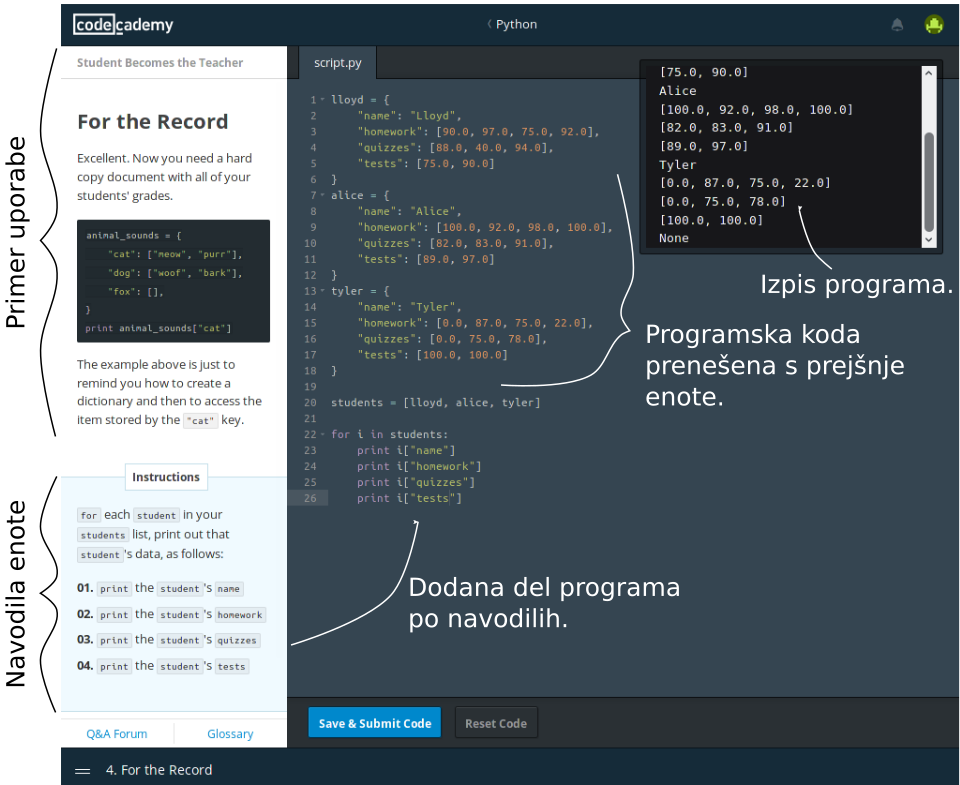
\includegraphics [width=0.65\linewidth, keepaspectratio =
   1] {./images/sc_web/codeacademy_IDE_02.png}
   \caption{Zaslonska slika
     \emph{\href{https://www.codecademy.com/}{Codeacademy}}
     \cite{web:codeacademy} urejevalnika z navodili in oknom za izpis
     v programu.}
    \label{fig:scr:web:codeacademy:ide}
\end{figure}

Vsaka tema je razdeljena na več enot, ki so sestavljene tako, da
postopoma dograjujejo program. Delo z prejšnje enote se samodejno
prenese naprej. Lahko povemo, da je \textbf{načelo postopnosti
upoštevano}. Pri nekaterih tematskih sklopih sledi najprej ponovitev že
naučenega. Na primer pri Temi \emph{Seznami in funkcije} najprej sledi
pregled osnovnega upravljanja z seznami in pisanjem funkcij.
Uporabniški vmesnik (slika \ref{fig:scr:web:codeacademy:ide}) je
urejen tako, da na desni strani imamo podano snov, ki je sestavljena s
\textbf{primerom določene programske strukture in navodili}, kaj
moramo dograditi v programu. Na levi strani imamo \textbf{urejevalnik
  besedil} v katerega pišemo programsko kodo. Urejevalnik zna barvati
programsko kodo in samodejno predviditi zamike besedila. V zgornjem
desnem kotu je \textbf{okno za izpis} v katerem se izpisujejo
\textbf{izhodni podatki} s programa in napake sintakse \textbf{Pyton
  tolmača}. Spodaj je gumb za \textbf{Shrani in oddaj programsko kode}
(\emph{ang. Save and Submit Code}).

Vsaka v uvodnem delu predstavi novo problematiko, ki jo potem čez
posamezne enote rešujemo. Vsebina je predstavljena
\textbf{problemsko}. Samo delo z \textbf{spletno aplikacijo za
  programiranje} poteka tako, da napišemo program, ki je zahtevan v
navodilih. Ko menimo, da imamo pravilno rešitev pritisnemo na gumb
\textbf{Shrani in oddaj programsko kodo.} Program preverja
\textbf{sintaktično} pravilnost. Napako program vrne nad gumbom za
oddajo programske kode, podrobna napaka \textbf{Pythonov tolmač} se
izpiše v \textbf{oknu za izpis}. Zatem sledi \textbf{semantično}
preverjanje pravilnosti rešitve naloge. V posamezni enoti program
samodejno vrši osnovno preverjanje programa, z točno določeni
rezultatom. Dokler test napisanega programa ne da pravega rezultata me
moremo nadaljevati na naslednjo enoto. Ko se nam zatakne, spletna
stran ponuja \textbf{forum} na katerem najdemo odgovor ali lahko
postavimo vprašanje. Forum je razdeljen na posamezne teme in enote,
tako da lahko hitro najdemo zahtevano vprašanje.

%Zbiranje dosežkov
Za uspešno premagovanje enot je uporabnik nagrajen z
\textbf{značkami}, ki so vidne na strani njegovega profila. Na tej
strani se beležijo tudi predelane vsebine. Spletni portal torej
uporablja nagrajevanje z \textbf{dosežki}.

Spletni portal ponuja tudi plačljive vsebine, čeprav je osnova
vsebinskih sklopov brezplačna. Za dostop do plačljivih storitev, za
ponujajo model zakupa z naročnino za ceno \textbf{19\$/mesec}. Za
naročnino uporabnik pridobi dostop do\textbf{ naslednjih dodatnih
  storitev}:

\begin{itemize}
\item personaliziran učni načrt;
\item dostop do kvizov;
\item dostop do realnih projektov;
\item dostop pomoči v živo preko sporočil.
\end{itemize}

Ugotovimo, da je spletni portal \textbf{pol plačljivi} in da dodatne
storitve, ki jih ponuja spletni portal niso potrebne za uporabo pri
pouku, saj vse omenjene dodatne storitve lahko zagotovi učitelj.

\subsubsection{Uporaba v šoli}
\label{sec:uporaba_v_soli}

Spletni portal nudi vsebine, ki so prilagojene za šole in uporabo v
šolah. V pregledu lahko ugotovimo, da za učitelje ponujajo naslednje
stvari:

\begin{itemize}
\item \textbf{trening za učitelje}, ki je dosegljiv le v ameriki;
\item \textbf{gradiva};
\item \textbf{sledenje napredku učencem};
\item \textbf{ura kode} (ang. \emph{Hour of code}).
\end{itemize}

Pod stran z \textbf{ gradivi} %(slika \ref{fig:scr:web:codeacademy:tr})
učitelju ponuja razdelane posamezne teme na enote podobno kot so
razdelane na glavni strani. Pod vsako enoto učitelj lahko preizkusi,
rešuje vaje. Večina enot ima pripravljene kvize, ki jih učitelj lahko
prav tako preizkusi in se pripravi na učno uro.


% \begin{figure}[h!]
%   \centering
%     \includegraphics [width=0.40\linewidth, keepaspectratio =
%    1] {./images/sc_web/codeacademy_tr_01.png}
%    \caption{Zaslonska slika
%      \emph{\href{https://www.codecademy.com/}{Codeacademy}}
%      \cite{web:codeacademy} pod strani z gradivi in tematskimi
%      sklopi.} %%NI ukazna vrstica temveč ...
%     \label{fig:scr:web:codeacademy:tr}
% \end{figure}

Kot so si zamislili avtorji spletnega portala so tematski sklopi in
posamezne enote med seboj prepletene in vodijo do posameznega
cilja. Zemljevid (slika \ref{fig:codeacademy:poster}) prikazuje
povezavo enot na posamezni stopnji in različne cilje. Za vsak tematski
sklop učitelj lahko prenese \textbf{pregled posamezne teme}, v kateri
so podrobneje zapisani učni cilji in so označene stopnje ki sovpadajo
z zemljevidom.

\begin{figure}[h!]
  \centering
    \includegraphics [width=1\linewidth, keepaspectratio =
   1] {./images/CAdemy-poster.pdf}
   \caption{Plakat z povezavami enot različnih tematskih sklopov po
     stopnjah, ki vodijo  do posameznih ciljev (\emph{ang. Level
       prograsion mapa}) \cite{web:codeacademy}.}
    \label{fig:codeacademy:poster}
\end{figure}

Ena izmed naprednih zmožnosti spletnega portala je \textbf{sledenje
  napredku učencem} \emph{ang. Students tracking}. Ta omogoča, da
učitelj učence z ustvarjenimi računi na spletnem portalu povabi v
razred. Določi tematske sklope katerim bo sledil. V pregledu (slika
\ref{fig:scr:web:codeacademy:tracking}) učitelj lahko opazuje napredek
posameznega učenca po enotah ali v povzetku za celotni
napredek. Napredek je prikazan z pikami različnih barv, ki
predstavljajo procente napredka pri posameznem tematskem sklopu. V tem
primeru \textbf{ne moremo} govoriti o \textbf{upravljanju razreda},
saj omogočeno le sledenje napredku in ne tudi komunikacija med
učiteljem in učenci, prav tako ni mogoče dodajati lasnih enot
oz. nalog. Pri samem ustvarjanju razreda, je učitelju delo zelo
olajšano, saj portal omogoča, da informacije o učencih ustvarjalec
razreda kopira direktno s programa podobnega kot je \textbf{Excel}. V
tabeli so podani podatki \textbf{ime, priimek, skupina, uporabniško
  ime}. Učenci za dostop do spletnega portala uporabijo uporabniško
ime, ki si ga izmisli učitelj ali sami ampak ga vnese učitelj in
geslo, ki je skupno za celotno učilnico. Prednost takega postopka
registracije je ta, da se učencem ni treba registrirati z lastnimi
podatki na primer s svojim email-om.

\begin{figure}[h!]
  \centering
    \includegraphics [width=0.65\linewidth, keepaspectratio =
   1] {./images/sc_web/codeacademy_tracking_01.png}
   \caption{Zaslonska slika
     \emph{\href{https://www.codecademy.com/}{Codeacademy}}
     \cite{web:codeacademy}. Prikazuje tabelo za sledneje napredku
     učencem.}
    \label{fig:scr:web:codeacademy:tracking}
\end{figure}

%Uporaba dosežkov
%Plačljive vsebine

\subsubsection{Povzetek}

\emph{\href{https://www.codecademy.com/}{Codeacademy}}
\cite{web:codeacademy} ima dobro razdelano vsebino, ki je na nekaterih
delih dokaj poglobljena. Sistematičnost, postopnost in problemski
pristop sta prav tako dobro zastavljeni. Portal ponuja številne
projektne vsebine in učenje programskih jezikov. Izbor teh je tak, da
ustreza današnjim spletnim tehnologijam in zahtevam. Znanje se omejuje
predvsem na učenje programiranja ter da se to znanje zna uporabiti v
praktične namene. Spletni portal ima nekatere vsebine in zmožnosti
plačljive, ampak ima zadostno število brezplačnih vsebin, ki omogočajo
normalno delo.

Zanemarjeno je znanje \textbf{Računalniške znanosti}, saj se med
spoznavanjem programskih jezikov in podatkovnih struktur ne uči
različnih algoritmov. Uči se bolj uporabo posameznih funkcij, ki so
vgrajene v programski jezik. Slaba stran spletnega portala je ta, da
je ves v \emph{angleškem jeziku}. Poleg tujega jezika so nekatera
navodila napisana dokaj kompleksno z obratno logiko in zahteva že
dobro poznavanje razumevanja sporočil tolmača in semantičnih napak, ki
se zgodijo v programu.

%Uporaba v šoli.

Spletni portal je v primeru učenja spletnih tehnologij, kot je
\textbf{HTML/CSS} je primeren za učence zadnje triade osnovne šole,
saj se ti omenjeno snov učijo pri izbirnem predmetu
\textbf{Računalniška omrežja}. V primeru učenja programskega jezika
\textbf{Python} spletni portal ponuja zahtevna znanja in je primeren
predvsem za srednje in višje šole.

Da bi mentor lahko spletni portal uporabljal pri pouku bi moral imeti
prevode navodil za posamezno temo in enoto. Vsekakor je možno izvesti
\emph{praktično vodeno delo}. Mentor lahko, spletni portal priporoča v
uporabo, kot za neobvezno dopolnilno dejavnost tistim, dijakom, ki
želijo razširiti znanje programiranja. Opozorimo, da jim lahko
priporoča le brezplačne vsebine.


\begin{osebnabox}[label={osebna:codeacademy}]{Codeacademy | \url{www.codeacademy.com}}
    \begin{tabular}{
  p{0.30\linewidth-2\tabcolsep} |
  p{0.70\linewidth-2\tabcolsep}  }
  \textbf{Vrsta vsebine} & \textbf{Napredna kombinirana vsebina}: primer,
                           navodilo(vodič), spletna aplikacija za programiranje.  \\
      \hline
  \textbf{Jezik spletne strani} &  Angleščina: da, slovenščina: ne,
                                  drugi: ne. \\
      \hline
  \textbf{Ponujena znanja} & Znanje prog. jezikov, druge vsebine. \\
      \hline
 \textbf{Programski jeziki} & \textbf{HTML+ CSS}, Java JavaScript, Jquery, PHP,
                              \textbf{Python}, Ruby \\
      \hline
  \textbf{Težavnostna stopnja} & 3/3 Osnovna šola, Srednja šola. \\
      \hline
   \textbf{Upoštevanje načel} & Upošteva načelo sistematičnosti: da,
      postopnosti: da, problemski pristop: da. \\
      \hline
  \textbf{Dosežki/Gamification} & Da (značke). \\
      \hline
  \textbf{Dodajanje lastnih vsebin} & Ne. \\
      \hline
  \textbf{Upravljanje razreda} &Da, ustvarjanje razreda in sledenje
                                 napredku učencem. \\
      \hline
  \textbf{Dostop vsebin} & Pol plačljiv (plačljivi so projekti, kvizi,
                           podpora v živo). \\
\end{tabular}
\end{osebnabox}

\subsection{Scratch}
\label{sec:scratch}

Spletni portal \emph{\href{https://scratch.mit.edu/}{Scratch}}
\cite{web:scratch} je spletna različica zelo popularnega programskega
jezika \textbf{Scratch}. Scratch je pri nas popularen predvsem v
\textbf{osnovnih šolah} in je zamenjal dolgo uporabljen \textbf{Logo}.

Razvoj samostojne namizne različice Scratcha se je končala pri verzi
1.4, od tu naprej je razvoj Scratcha potekal za spletno
različico. Spletna različica je narejena na osnovi zaprtega
\textbf{Adobe Flash}. Za poganjanje Scratch v spletnem brskalniku
potrebujemo vtičnik \textbf{Flash}.

Ko prvič naložimo spletni portal
\emph{\href{https://scratch.mit.edu/}{Scratch}} (slika
\ref{fig:web:scratch:main}) lahko ugotovimo, da ponuja naslednje
funkcionalnosti:

\begin{figure}[h!]
  \centering
    \includegraphics [width=0.90\linewidth, keepaspectratio =
   1] {./images/sc_web/scratch_mainP-v01.png}
   \caption{Zaslonski posnetek glavne strani
     \emph{\href{https://scratch.mit.edu/}{Scratch}}
     \cite{web:scratch}.}
    \label{fig:web:scratch:main}
\end{figure}

\begin{itemize}
\item ustvarjanje programov (Orodje Scratch);
\item deljenje ustvarjenih programov;
\item raziskovanje narejenih programov, drugih uporabnikov;
\item forum za diskusije;
\item pomoč pri uporabi
\end{itemize}

Scratch smo po vrsti vsebine umestili med \textbf{spletne aplikacije
  za programiranje} oz. smo ga predstavili kot samostojno
\textbf{orodje}, kajti vse učne vsebine, so narejene iz razloga učenja
uporabe orodje in spoznavanjem zmožnosti programskega jezika. Govorimo
lahko vseeno o spletnem portalu, saj ta ima vse za uspešno uporabo
orodja in omogoča vso funkcionalnost, ki jo potrebuje neka spletna
skupnost.

\subsubsection{Uporaba Scratcha}
\label{sec:uporaba_scratcha}

Scratch omogoča ustvarjanje animacij, predstavitev in iger. Namenjen je
8 do 16 let starim, vendar ne predstavlja nobene omejitve na zgornji
meji starosti. Preveden je v številne jezike med njimi je tudi
\textbf{slovenščina} \cite{web:scratch:about}.

Če smo v preteklosti že uporabljali namizno različico Scratcha, nam
spletna različica (slika \ref{fig:web:scratch:orodje}) nebo predstavljala
nobenih težav, saj je postavitev skoraj enaka kot je bila
namizna. Osnovni princip delovanja je tak, da na \emph{oder} (slika
\ref{fig:web:scratch:orodje}) postavljamo različne \emph{like}. Vsak
lik, ki ga dodamo z knjižnice ali ga naložimo sami, je predstavljen
kot svoj objekt in vsakemu posebej dodajamo programsko kodo, ki jo
sestavljamo iz različnih \emph{gradnikov}. V samem orodju lahko
dorisujemo k že obstoječim likom ali ustvarjamo nove. Dodajamo lahko
tudi zvok, ki ga posnemamo sami ali ga izberemo iz knjižnice zvokov.
Programsko kodo lepimo skupaj oz. sestavljamo podobno kot lego
kocke. Gradniki so oblikovani tako, da se sklopijo samo, ki se morajo.

\begin{figure}[h!]
  \centering
    \includegraphics [width=0.90\linewidth, keepaspectratio =
   1] {./images/sc_web/scratch_orodje-v021.png}
   \caption{Zaslonska slika
     \emph{\href{https://scratch.mit.edu/}{Scratch}}
     \cite{web:scratch}.}
    \label{fig:web:scratch:orodje}
\end{figure}

\textbf{Vodiče} v Scratchu najdemo na desnem robu (slika
\ref{fig:web:scratch:orodje}). Vodiči so sestavljeni tako, da
uporabnika postopoma vodijo skozi gradnjo programa. S tem je
zagotovljena \textbf{postopnost}. Posamezen korak v vodiču je
sestavljen iz besedila in animiranega poteka dela.

\subsubsection{Deljenje in raziskovanje projektov}
\label{sec:deljenje_vsebin}

Vsak uporabnik, ki se registrira na spletnem portalu ima dostop do
svojega profila. Na svoji strani se samodejno shranjujejo projekti, ki
smo jih izdelovali in jih od tu lahko ponovno naložimo za
urejanje. Vse projekte lahko delimo z drugimi. Vsak projekt ima svojo
pod stran na kateri določamo nastavitve za \emph{deljenje} (slika
\ref{fig:web:scratch:deljenje}). Na strani lahko dodamo \emph{navodila
  za program} in \emph{zapiske in zasluge}, prav tako določamo, če
želimo projekt deliti ali ne.

\begin{figure}[h!]
  \centering
    \includegraphics [width=0.50\linewidth, keepaspectratio =
   1] {./images/sc_web/scratch_deljenje-v01o.png}
   \caption{Pod stran za deljenje projekta na
     \emph{\href{https://scratch.mit.edu/}{Scratch}}
     \cite{web:scratch}.}
    \label{fig:web:scratch:deljenje}
\end{figure}

Če je omogočeno da lahko delimo vsebine je na spletnem portalu tudi
dobro poskrbljeno za \textbf{raziskovanje projektov} drugih
uporabnikov. Pod zavihkom \textbf{razišči \emph{(ang. Explor)}}
najdemo številne projekte, ki razdeljeni v kategorije. Tu lahko črpamo
številne ideje in si najljubše projekte shranimo tudi na svojem
profilu.

\subsubsection{Povzetek}
\label{sec:scratch_povzetek}

\textbf{Učni načrt} v slovenski osnovni šoli ne obveznega izbirnega
predmeta \textbf{Računalništvo }je prilagojen prav za uporabo
Scratcha. Čeprav z dobro pripravljenimi vodiči spoznavamo tudi na
primer vejitve, v Scratchu pod gradniki \emph{Kontorla}, si učitelj
mora pripraviti in prilagoditi vsebino za uresničevanja učnega načrta
sam. Na spletni strani lahko črpamo številne ideje iz projektov drugih
uporabnikov.

Za slabost spletne različice štejemo lahko edino stvar in to, da
je narejen z zaprto tehnologijo \textbf{Adobe Flash}, kar pomeni, da
si uporabnik mora naložiti vtičnik Flash za spletni brskalnik. Vtičnik
Flash uradno podpira le nekatere komercialne operacijske sisteme in
njegovo vlogo zamenjuje vedno boljše zmožnosti samih spletnih
brskalnikov z tehnologijo \textbf{HTML5 + CSS + JS}.

\begin{osebnabox}[label={osebna:scratch}]{Scratch | \url{https://scratch.mit.edu}}
    \begin{tabular}{
  p{0.30\linewidth-2\tabcolsep} |
  p{0.70\linewidth-2\tabcolsep}  }
  \textbf{Vrsta vsebine} & Spletna aplikacija za prog. \\
      \hline
  \textbf{Jezik spletne strani} & Scratch: angleščina: da, slovenščina: da,
                                  drugi: da. Spletni portal:
                                  angleščina: da, drugi: ne\\
      \hline
  \textbf{Ponujena znanja} & Vodiči za spoznavanje uporabe Scratch in pomoč \\
      \hline
 \textbf{Programski jeziki} & Scratch \\
      \hline
  \textbf{Težavnostna stopnja} & Osnovna šola \\
      \hline
   \textbf{Upoštevanje načel} & Problemski pristop: ne,
                                sistematičnost: ne, postopnost: da (Vodič). \\
      \hline
  \textbf{Dosežki/Gamification} & Ne. \\
      \hline
  \textbf{Dodajanje lastnih vsebin} & Ne. \\
      \hline
  \textbf{Upravljanje razreda} & Ne. \\
      \hline
  \textbf{Dostop vsebin} & Brezplačen. \\

\end{tabular}
\end{osebnabox}

\subsection{repl.it}
\label{sec:repl.it}

\textbf{\emph{\href{https://repl.it/}{Repl.it}}} \cite{web:replIT} je še ena
\textbf{spletna aplikacija za programiranje}. Podjetje, ki spletno
stran ustvarja je tržno osredotočeno na ponujanje \textbf{aplikacijski
  programski vmesnik - APV} ali (\emph{ang. application programming
  interface - \textbf{API}}). Njihov APV uporabljajo številni spletni
portali kot je na primer
\emph{\href{freecodecamp}{https://www.freecodecamp.com}}
\cite{web:freecodecamp} in nekateri drugi plačljivi spletni
portali. Na spoji strani ponujajo prost dostop do spletne aplikacije
za programiranje \ref{}.

\begin{figure}[h!]
  \centering
    \includegraphics [width=0.65\linewidth, keepaspectratio =
   1] {./images/sc_web/replIT_main-v01.png}
   \caption{Zaslonska slika spletne aplikacije za programiranje
     \emph{\href{https://repl.it/}{repl.it}} \cite{web:replIT}.}
    \label{fig:web:replIT}
\end{figure}

Aplikacija ponuja številne programske jezike kot je \textbf{Python3,
  Ruby, JavaScript, HTML, CSS, C\#, JAVA} in še mnoge druge. Vsako nova
pojava spletne aplikacije predstavlja novo sejo. Po registraciji na
spletnem portalu lahko shranjujemo posamezne seje. Posamezno sejo
lahko \textbf{tudi delimo} preko spletne povezave. \textbf{Urejevalnik
  besedil} omogoča barvanje rezerviranih besed programske kode in ima napredno
\textbf{možnost ponujanja predlogov} za samo dokončevanje izpisa
rezerviranih besed in funkcij programskega jezika.

\subsubsection{Ustvarjanje razredov in nalog}
\label{sec:ustvarjanje_raz_nalog}

Spletni portal skorja, da ni vreden omembe z \textbf{vsebinskega
  vidika} tudi kot spletna aplikacija me predstavlja nekih posebnih
funkcij, ki jih nebi imele tudi nekatere druge spletne aplikacije. Ima
pa spletni portal eno veliko prednost saj omogoča \textbf{ustvarjanje
  razredov}. Mentor lahko ustvarja razred in v njega povabi dijake ter
samodejno dodaja oz. \textbf{ustvarja lastne naloge}
\ref{fig:web:replIT:assigment}. Dijake v razred povabi z dodajanjem
email-ov v seznam. Dijaki se ne potrebujejo registracije, z povezavo,
ki so jo dobili na email se prijavijo v razred. Mentor v načinu
ustvarjanja naloge, doda lastna navodila in začetno programsko kodo. V
naslednjem koraku se mentor lahko odloči ali bo pravilnost naloge
preverjal sam ali po dodal avtomatski preizkus programske kode. V
avtomatskem načinu mora podati primer vhodnih podatkov in rezultat
izhoda.

 V razredu dijaki vidijo seznam nalog. Naloge se dijakom
prikazane z navodili, ko so dijaki zadovoljni s svojo rešitvijo,
nalogo oddajo. Mentorju se status naloge pri dijaku spremeni na
\emph{oddano} in sedaj mentor nalogo lahko pregleda, poda komentar in
jo označi lahko označi kot \emph{opravljeno}.

\begin{figure}[h!]
  \centering
    \includegraphics [width=0.75\linewidth, keepaspectratio =
   1] {./images/sc_web/replIT_assigment-v01.png}
   \caption{Zaslonska slika pogleda mentorja v načinu priprave naloge
     \cite{web:replIT}.}
    \label{fig:web:replIT:assigment}
\end{figure}

\subsubsection{Povzetek}
\label{sec:povzetek:replIT}

Ta spletna aplikacij za programiranje, ponuja mentorjem računalniških
vsebin osnovno orodje za ustvarjanje razredov in nalog ter
komunikacijo z dijaki. Pri tem uporablja osnovne zmožnosti brez
pretirane kompleksnosti. Sam spletni portal ne ponuja nobene vsebine,
kar je sovje vrstna prednost, saj lahko mentor prilagodi naloge učnemu
načrtu in to v svojem jeziku.

\begin{osebnabox}[label={osebna:replIT}]{Repl.it | \url{https://repl.it/}}
    \begin{tabular}{
  p{0.30\linewidth-2\tabcolsep} |
  p{0.70\linewidth-2\tabcolsep}  }
  \textbf{Vrsta vsebine} & Spletna aplikacija za prog. \\
      \hline
  \textbf{Jezik spletne strani} & angleščina: da, slovenščina: ne,
                                  drugi: ne. \\
      \hline
  \textbf{Ponujena znanja} & Ne ponuja nobene vsebine\\
      \hline
 \textbf{Programski jeziki} & Python3,
  Ruby, JavaScript, HTML, CSS, C\#, JAVA in drugi\\
      \hline
  \textbf{Težavnostna stopnja} & Srednja šola.\\
      \hline
   \textbf{Upoštevanje načel} & Problemski pristop: ne,
                                sistematičnost: ne, postopnost: ne (Vodič). \\
      \hline
  \textbf{Dosežki/Gamification} & Ne. \\
      \hline
  \textbf{Dodajanje lastnih vsebin} & Da. Ustvarjanje razreda in nalog
                                      ter komunikacija z dijaki. \\
      \hline
  \textbf{Upravljanje razreda} & Da. \\
      \hline
  \textbf{Dostop vsebin} & Brezplačen. \\

\end{tabular}
\end{osebnabox}

\subsection{Tutorialspoint}
\label{sec:tutorials_point}

\emph{\href{http://www.tutorialspoint.com/}{Tutorials point}}
\cite{web:tutorialspoint} je eden izmed velikih portalov, ki ponujajo
obsežne in zahtevne vodiče tehničnih in ne tehničnih vsebin. Na
spletno je vodičev veliko, tega smo izpostavili iz razloga, ker ponuja
ogromno \textbf{vsebin programiranja in računalniške znanosti}, vsi
primeri v vodičih imajo \textbf{možnost preizkusa} in razvito imajo
lastno \textbf{spletno aplikacijo za programiranje}, ki ima veliko
zmožnosti, nekatere značilne za namizne \textbf{IDE}.

Spletni portal ponuja knjižnico vodičev (\ref{fig:web:tutpoint:lib})
različnih vsebinskih sklopov. Z slike je razvidno, da je zares
obsežna.

\begin{figure}[h!]
  \centering
    \includegraphics [width=0.75\linewidth, keepaspectratio =
   1] {./images/sc_web/tutpoint_lib-v01.png}
   \caption{Del seznama oz knjižnica vodičev, ki ga ponuja spletna
     stran \emph{\href{http://www.tutorialspoint.com/}{Tutorials
         point}} \cite{web:tutorialspoint}.}
    \label{fig:web:tutpoint:lib}
\end{figure}

Vsebinsko si smo pregledali vodič za \textbf{Python3} (slika
\ref{fig:web:tutpoint:tut01}). Vodiči so oblikovani tako, da na desni
strani najdemo kazalo vsebine, v sredinskem delu je razložena snov z
primeri.

%Dodaj besedilo v sliko.
\begin{figure}[h!]
  \centering
    \includegraphics [width=0.65\linewidth, keepaspectratio =
   1] {./images/sc_web/tutpoint_tutP3-v01.png}
   \caption{Zaslonski izrez vodiča za Python3. S like je razvidno
     kazalo in gumb za \textbf{Preizkus!} \cite{web:tutorialspoint}.}
    \label{fig:web:tutpoint:tut01}
\end{figure}

Nekatere od primerov lahko tudi preizkusimo, z klikom na gumb
\textbf{Preizkusi (\emph{ang. Try it})}, se nam na isti strani odpre
podokno (slika \ref{fig:web:tutpoint:tut02}). Kodo v urejevalniku
lahko spreminjamo in ponovno zaženemo.

%Dodaj besedilo v sliko.
\begin{figure}[h!]
  \centering
    \includegraphics [width=0.65\linewidth, keepaspectratio =
   1] {./images/sc_web/tutpoint_tutP3-v02.png}
   \caption{Pod okno za preizkus primera programske kode
     \cite{web:tutorialspoint}.}
    \label{fig:web:tutpoint:tut02}
\end{figure}

\subsubsection{Coding ground}
\label{sec:coding_ground}

Kot smo že omenili spletni portal kot orodje ponuja lastno spletno
aplikacijo za programiranje. Spletna aplikacija se imenuje
\emph{\href{http://www.tutorialspoint.com/codingground.htm}{Codingground}}
\cite{web:tutorialspoint:codingground}. Na uvodni strani õrodja (slika
\ref{fig:web:tutpoint:cg-pl}) smo odkrili, številnost ponujenih
\textbf{programskih jezikov}, ki sovpadajo s številnimi vodiči, ki jih
ponuja spletni portal.

\begin{figure}[h!]
  \centering
    \includegraphics [width=0.65\linewidth, keepaspectratio =
   1] {./images/sc_web/tutpoint_cg-pl-v01.png}
   \caption{Del seznama različnih programskih jezikov katere lahko
     uporabljamo z spletno aplikacijo za programiranje
     \emph{\href{http://www.tutorialspoint.com/codingground.htm}{Codingground}}
     \cite{web:tutorialspoint:codingground}.}
    \label{fig:web:tutpoint:cg-pl}
\end{figure}

Razporeditev spletne aplikacije (slika \ref{fig:web:tutpoint:cg})je
taka, da na levem robu imamo seznam datotek v korenskem imeniku, v
sredinskem delu je urejevalnik besedil, nad urejevalnikom najdemo
menijsko vrstico in na dnu strani je \textbf{ukazna vrstica}, v kateri
lahko zaganjamo napisano programsko kodo. V njej se izpisujejo tudi
povratne informacije tolmača in izhod programske
kode. \textbf{Urejevalnik besedil} besedil omogoča barvanje kode
rezerviranih besed in nastavljanje barvne sheme
urejevalnika. Urejevalnik omogoča še samodejno zamikanje programske
kode, ko je to potrebno. \textbf{Shranjevanje in uvažanje projektov v
  oblak}, lahko smatramo kot eno izmed prednosti te spletne
aplikacije. \emph{\href{http://www.tutorialspoint.com/codingground.htm}{Codingground}}
lahko nastavimo, da se poveže s oblačnimi shrambami kot so
\textbf{Dropbox, Google Drive, Onedrive} in s sistemom za objavljanje,
upravljanje verzij in kolaboracijo \textbf{Git}. Seveda lahko projekt
naložimo neposredno z računalnika in ga seveda tja tudi
shranimo. Prednost oblačnega shranjevanja je ta, da na programiramo
lahko od koder koli in z katerim orodjem želimo. če je to spletna
aplikacija ali namizna. Spletna aplikacija omogoča tudi upravljanje z
datotekami. Lahko ustvarimo, preimenujemo in brišemo datoteke ali
imenike. To lahko počnemo z \textbf{menija (\emph{file}) ali ukazne
  vrstice}. Vsak projekt lahko delimo preko neposredne kratke
\textbf{url povezave}, kot smo to že videli pri drugih spletnih
portalih.


\begin{figure}[h!]
  \centering
    \includegraphics [width=0.65\linewidth, keepaspectratio =
   1] {./images/sc_web/tutpoint_cg-v01.png}
   \caption{Spletna aplikacija za programiranje -
     \emph{\href{http://www.tutorialspoint.com/codingground.htm}{Codingground}}
     \cite{web:tutorialspoint:codingground}.}
    \label{fig:web:tutpoint:cg}
\end{figure}

\subsubsection{Povzetek}
\label{sec:povzetek_tutpoint}

Vsebina vodičev je zelo tehnična in deluje kot zelo okrnjen povzetek
uradne reference za določen programski jezik. Kot taka je predvsem
primerna za programerje začetnike, ki se želijo poučiti o določenem
programskem jeziku, vendar že poznajo osnovne koncepte
programiranja. Velik plus je vsekakor preizkus programske
kode. Vodiče lahko priporočimo kot kratko referenco nekemu
programskemu jeziku.

S pravo nastavitvijo, spletna aplikacija omogoča, da dijaki imajo
programsko kodo in snov, ki jo v nekem trenutku predelujejo povsod na
voljo. S pomočjo shranjevanja in deljenja projektov lahko mentor
uporabi spletno aplikacijo kot glavno orodje za učenje računalništva
in programskega jezika. Mentor mora pripraviti sistem za izmenjavo
navodil, programske kode, in rešitev dijakov. To lahko stori uporabo
kratkih url povezav. Urejevalnik besedil bi lahko ponujal kakšno
zmožnost več kot jo, vendar zadosti osnovnim potrebam pisanja
programske kode.


\begin{osebnabox}[label={osebna:replIT}]{Repl.it | \url{https://repl.it/}}
    \begin{tabular}{
  p{0.30\linewidth-2\tabcolsep} |
  p{0.70\linewidth-2\tabcolsep}  }
  \textbf{Vrsta vsebine} & Osnova kombinirana vsebina: vodič in
                           preizkus programske kode. Posebej spletna
                           aplikacija za učenje programiranja:
                           Codingground \\
      \hline
  \textbf{Jezik spletne strani} & angleščina: da, slovenščina: ne,
                                  drugi: ne. \\
      \hline
  \textbf{Ponujena znanja} & Znanja prog. Jezikov + druge
                             vsebine. Vodiči s številnih področij. \\
      \hline
 \textbf{Programski jeziki} & Velika knjižnica prog. Jezikov in vsebin
                              rač. Znanosti. \\
      \hline
  \textbf{Težavnostna stopnja} & Srednja šola.\\
      \hline
   \textbf{Upoštevanje načel} & Problemski pristop: ne,
                                sistematičnost: ne, postopnost: da (Vodič). \\
      \hline
  \textbf{Dosežki/Gamification} & Ne. \\
      \hline
  \textbf{Dodajanje lastnih vsebin} & Da. Ustvarjanje podporne
                                      programske kode v spletni
                                      aplikaciji za prog., vendar brez
                                      navodil in deljenje vsebine.  \\
      \hline
  \textbf{Upravljanje razreda} & Na. \\
      \hline
  \textbf{Dostop vsebin} & Brezplačen. \\

\end{tabular}
\end{osebnabox}

\subsection{Code combat}
\label{sec:code_battle}

Spletni portal \emph{\href{https://codecombat.com/}{Code combat}}
\cite{web:codecombat} je mešanica med igranjem igre in pisanjem
programske kode. V predstavitvi spletne strani pravijo naslednje,
\emph{``Če se želiš naučiti programirati, moraš napisati veliko
  programske kode''} \cite{web:codecombat:about}. Spletna stran ponuja
tri načine registracije, ustvarite lahko \textbf{navaden},
\textbf{učiteljski} ali \textbf{učencev}, račun. V pregledu strani smo
uporabili prijavo z navadnim računom, prav tako smo povzeli posebnosti
ostalih dveh računov.

\subsubsection{Upravljanje razreda}
\label{sec:upravljanje_razreda}

Spletni portal omogoča upravljanje razredov. Razrede upravlja
\textbf{učitelj}. Portal ima prilagojeno učno snov za tri stopnje po
ameriškem \textbf{K-12} sistemu. Kot smo še primerjali šolske sisteme
lahko povemo, da so stopnje po starosti v slovenski šole prilagojene
na naslednje \textbf{osnovno šolo (2.triado in 3. triado) in srednjo
  šolo}.

\subsection{Codingame}
\label{sec:codingame}




\section{Ovrednotenje izbranih spletnih portalov in njihove posebnosti}
\label{sec:pregled_spletnih_portalov}


\section{Možni načini uporabe spletnih portalov pri pouku}
\label{sec:načini_uporabe_sp}

%Nekakšen povzetek zgornjih člankov. Vprašanja za naprej.
\subsection{Prednosti pri uporabi SPUP v šoli }
\label{sec:Prednosti_pri_uporavi_SPUP}

% Po pregledu, ki se ukvarjajo z učenjem programiranja lahko
% ugotovimo, da je samo učenje programiranja tanko staro kot prvi
% program, ki je bil kdaj koli napisan.

% NOTE: Razlikovati moramo med kodiranjem in reševanjem problemov
% Začetne misli o učenju programiranja.

% NOTE: Zanima nas naslednja vprašanja:
% NOTE: * Kaj so spletni portali za učenje programiranja?
% NOTE: * Zakaj in kje je smiselno uporabljati spletne portale za
% NOTE:   učenje programiranja.
% NOTE: * Prednosti spletnih portalov in slabosti?
% NOTE: * Kako so spletni portali zgrajeni?
% NOTE: * Katere so različne vrste spletnih portalov (Kategorije) in
% NOTE:   katere bodo nas zanimale?
% NOTE: *

% Kateri tradicionalni spletni portali? Preveri?
% Ali že tu pisati, da v tem primeru gre za učenje na daljavo?!
Tradicionalni spletni portali v izobraževanju, kot so \textbf{moodle},
nikoli niso popolnoma izkoristili zmožnosti uporabe, ki jih ponujajo
nove internetne in komunikacijske tehnologije. Večinoma so se
uporabljale le kot podaljšana roka obstoječim metodam
poučevanja. Uporabljale so se za objavo gradiv in spletno prijavo za
oddajo nalog. Takšni sistemi ne zagotavljajo izboljšav kvalitete
poučevanja programiranja \cite{ITaLCP_DistanceEdu}.

Strnimo nekatere značilnosti težav novincev.

\begin{itemize}
\tightlist
\item Težave pri namestitvi in nastavitvah programske opreme,
  prevajalnika in razvojnega okolja (OUHK, QUTA ).
\item Dostop do mentorjev zaradi časovne dostopnosti in Komunikacija v
  primeru izobraževanja na daljavo (OUHK, QUTA).
\item Uporaba urejevalnika besedil (QUTA).
\item Razumevanje programskih vprašanj in uprabe sintakse jezika pri
  pisanj programske kode (QUTA).
\item Uporoaba tehnik razhroščevanje (QUTA).
\item Razumevanje napak prevajalnika (QUTA).
\item Razumevanje osnovnih programskih koceptov, slabo vpliva na
  reševanje koceptov (US).
\end{itemize}

S težavami novince se lahko poistovetijo tudi učenci in dijaki, ki začnejo z
učenjem programiranja. Rešitve, ki jih je uporaba SPUP prinesla na
univerze lahko prenesemo na uporabo v osnovno in srednjo
šolo. Naštejemo lahko nekatere prednosti, ki bi jih taka uporaba lahko
imela.

\subsubsection{Namestitev programske opreme}
\label{sec:Namestitev_programske_opreme}

Med prvimi prednostmi je sigurno namestitev potrebne programske
opreme. Učitelju praktično ni potrebno nameščati nobenega urejevalnika
besedil, IDE, niti prevajalnika ali tolmača. Prav tako ni potrebe po
nastavljanju sistemskih poti, ki jih mnogi prevajalniki zahtevajo.

Uporaba SPUP je neodvisna od uporabe operacijskega sistema. Vsaka
naprava, na kateri lahko poganjamo spletni brskalnik omogoča uporabo
SPUP.

Velika prednost, da ni potrebe po instalaciji programske opreme je
tudi za učence, saj jim doma ni potrebno nalagati nobenega
programa. Na tem mestu bi poudarili, da učitelj mora biti previden pri
dajanju domače naloge z uporabo računalnika. Zares se mora prepričati,
da to zmožnost imajo vsi učenci. Najbolje je da vso dodatno delo, ki
ga učitelj predvidi lahko učenci opravijo v šolski računalniški
učilnici.

\subsubsection{Seznanjanje s programsko opremo}
\label{sec:Seznanjanje_s_prog_opremo}

Za učence ni potrebe, da bi spoznavali urejevalnik besedil ali
IDE. Spoznavanja programskega jezika in reševanje problemov se lahko
lotijo nemudoma.


\subsubsection{Pisanje programa od začetka do konca ni potrebno}
\label{sec:pisanj_celega_progama}

Večina spletnih portalov, ki ponujajo vsebine, imajo programske naloge
pripravljene tako, da uporabnik mora vnesti le del programske kode. Za
novinca, to pomeni, da se koncentrira le na nalogo in del sintakse, ki
jo v danem trenutku potrebuje, da reši zadano nalogo. To prednost smo
že spoznali na SPUP avstralske univerze, kjer so uporabili, tip
naloge, zapolni prazna mesta \cite{thesisAWebP}.

%To mogoče ne spada sem saj je bolj specifićen feature.
\subsubsection{Nagrajevanje z dosežki}
\label{sec:nagrajevanje_s_dosežkov}



\section{Ovrednotenje izbranih spletnih portalov in njihove posebnosti}
\label{sec:pregled_spletnih_portalov}


\section{Možni načini uporabe spletnih portalov pri pouku}
\label{sec:načini_uporabe_sp}



%%% Local Variables:
%%% mode: latex
%%% TeX-master: "diploma"
%%% End:
